Motorul statistic este realizat prin integrarea unei componente care comunica cu o instanta de R 
( \url{http://www.r-project.org/} ), 
disponibila pentru prelucrari statistice.
Aceasta se bazeaza pe o interfata Java-to-R 
(implementata via JNI, Java Native Interface), 
o librarie numita rJava ( \url{http://www.rforge.net/rJava/} ).

In cadrul proiectului Spring a fost dezvoltat un controller si un serviciu ce instantiaza si utilizeaza rJava 
pentru evaluarea de expresii, comenzi, functii 
(acestea fiind construite pe baza datelor importate in baza de date, ce corespund fiecarui studiu). 
Sunt posibile operatii multiple asupra unui set de [1..N] variabile ce apartin unui studiu.
A fost dezvoltat un set de functii parametrizate in limbajul R, ce sunt incarcate si apelate la runtime 
(parametrii functiilor fiind de exemplu nume de variabile, categorii, etichete, valori de missing, valori propriu-zise ale unei variabile etc.);
unele dintre aceste functii construiesc raspunsul pe care aplicatia il trimite mai departe catre clientul ExtJS (in format JSON), 
iar acesta le afiseaza in mod structurat (inclusiv tabele, grafice).

Mai jos este prezentata o imagine a modulului de acces la date, in care se pot vedea (in partea dreapta-jos) 
si rezultatele obtinute de la motorul statistic pentru analiza unei variabile.

\medskip
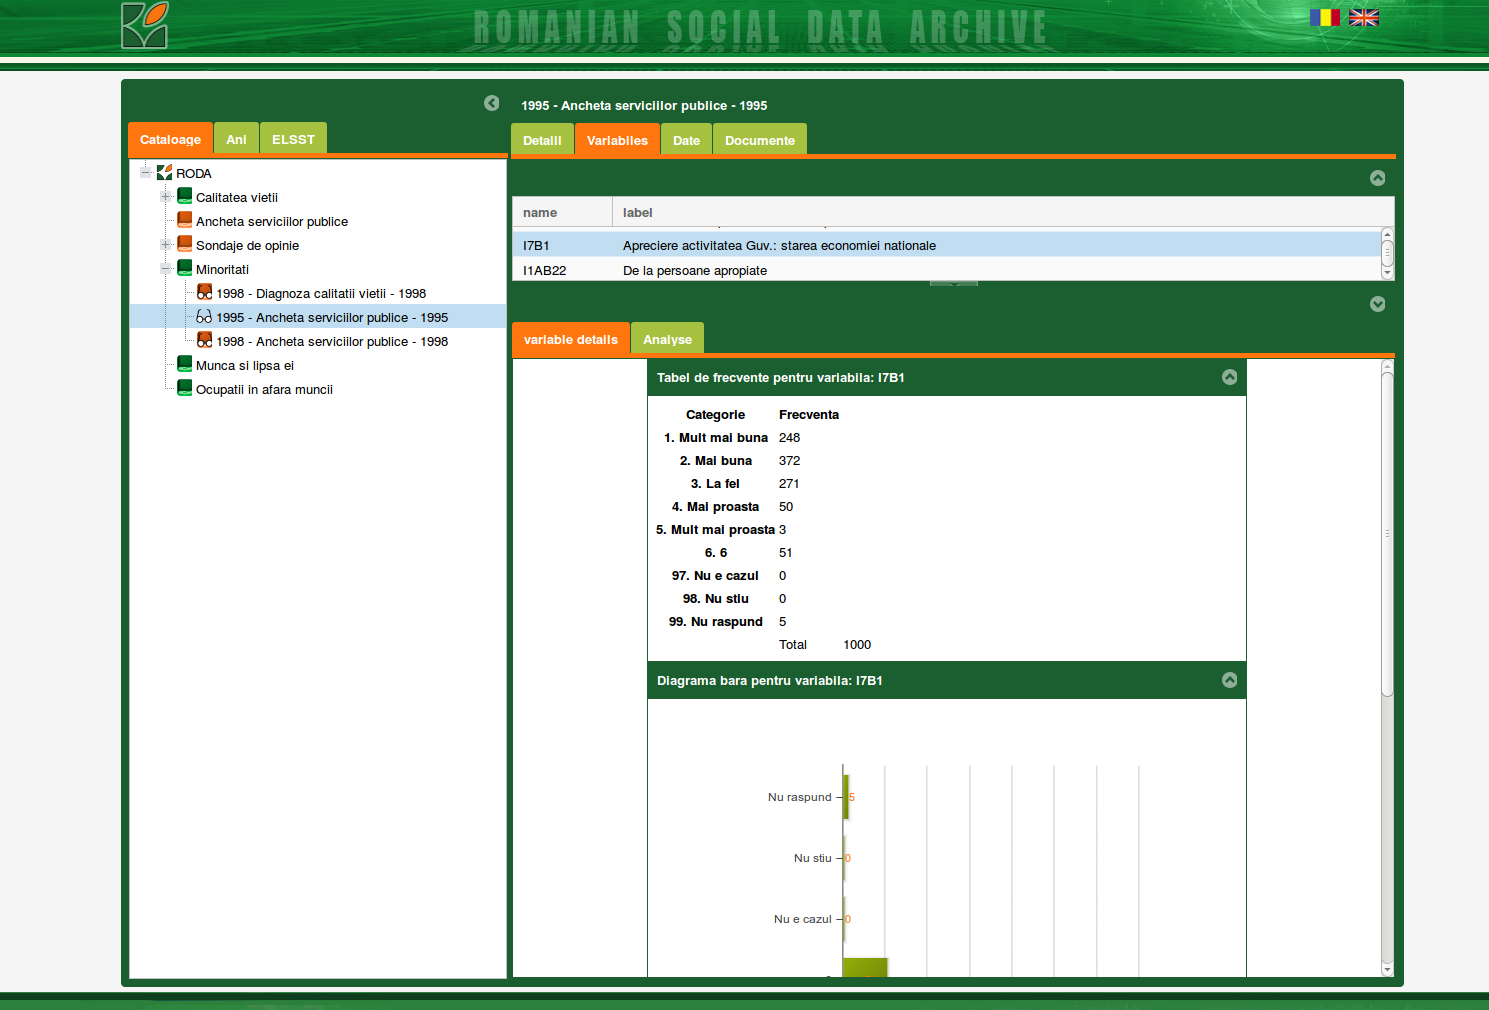
\includegraphics[width=\textwidth]{img/Screenshot-statistics}
